%
% The first command in your LaTeX source must be the \documentclass command.
\documentclass[sigconf,nonacm=true]{acmart}
\usepackage{titletoc}
\usepackage{color, colortbl}
\usepackage{array}
\definecolor{Gray}{gray}{0.9}


\newenvironment{my_itemize}{
	\begin{itemize}
		\setlength{\itemsep}{1pt}
		\setlength{\parskip}{0pt}
		\setlength{\parsep}{0pt}}
	{\end{itemize}
}

\newenvironment{my_enumerate}{
	\begin{enumerate}
		\setlength{\itemsep}{0pt}
		\setlength{\parskip}{0pt}
		\setlength{\parsep}{0pt}}
	{\end{enumerate}
}

\setlength{\parindent}{0pt}

% Online Latex Word Count:
% https://app.uio.no/ifi/texcount/online.php

%
% defining the \BibTeX command - from Oren Patashnik's original BibTeX documentation.
\def\BibTeX{{\rm B\kern-.05em{\sc i\kern-.025em b}\kern-.08emT\kern-.1667em\lower.7ex\hbox{E}\kern-.125emX}}
    
% Rights management information. 
% This information is sent to you when you complete the rights form.
% These commands have SAMPLE values in them; it is your responsibility as an author to replace
% the commands and values with those provided to you when you complete the rights form.
%
% These commands are for a PROCEEDINGS abstract or paper.


%
% These commands are for a JOURNAL article.
%\setcopyright{acmcopyright}
%\acmJournal{TOG}
%\acmYear{2018}\acmVolume{37}\acmNumber{4}\acmArticle{111}\acmMonth{8}
%\acmDOI{10.1145/1122445.1122456}

%
% Submission ID. 
% Use this when submitting an article to a sponsored event. You'll receive a unique submission ID from the organizers
% of the event, and this ID should be used as the parameter to this command.
%\acmSubmissionID{123-A56-BU3}

%
% The majority of ACM publications use numbered citations and references. If you are preparing content for an event
% sponsored by ACM SIGGRAPH, you must use the "author year" style of citations and references. Uncommenting
% the next command will enable that style.
\citestyle{acmauthoryear}


%
% end of the preamble, start of the body of the document source.
\begin{document}

%
% The "title" command has an optional parameter, allowing the author to define a "short title" to be used in page headers.
\title{Visualizing A Connection Between Electrical Generation and Surface Temperatures and CO$_2$ Emissions \\ CSE6242 - Team 52}

%
% The "author" command and its associated commands are used to define the authors and their affiliations.
% Of note is the shared affiliation of the first two authors, and the "authornote" and "authornotemark" commands
% used to denote shared contribution to the research.


\author{James Bonifield}
\affiliation{\institution{}}
\email{jbonifield3@gatech.edu}

\author{Diego Carvallo}
\affiliation{\institution{}}
\email{dcarvallo3@gatech.edu}

\author{Christopher Comfort}
\affiliation{\institution{}}
\email{ccomfort3@gatech.edu}

\author{Wesley Smith}
\affiliation{\institution{}}
\email{wsmith42@gatech.edu}

% The abstract is a short summary of the work to be presented in the article.
%\begin{abstract}
%This proposal describes our Spring 2019 CSE6242 Team Project.  In this proposal we will be answering Heilmeier's questions, describe what we plan to do, how we will do it, the tools we plan to use and how our approach improves on current state of the art, why we believe it will succeed, and what differences will it make.  \\
%\end{abstract}
% This command processes the author and affiliation and title information and builds
% the first part of the formatted document.
\maketitle
\section{Defining Our Problem Space:}
We will use the following datasets to develop analytical tools for presenting geographic and time-based visualizations:
\begin{my_enumerate}
	\item Berkely Earth - temperature data \cite{Berkeley_Earth_temp_rohde2013berkeley} [\href{http://berkeleyearth.org/data/}{\color{blue}link}]
	\item CDIAC - CO$_2$ emissions \cite{Foosil_fuel_burning_andres1997geographic}
	 [\href{https://cdiac.ess-dive.lbl.gov/epubs/ndp/ndp058/ndp058_v2016.html}{\color{blue}link}]
	\item EIA-923 - US Power Generation Statistics [\href{https://www.eia.gov/electricity/data/eia923/}{\color{blue}link}]
\end{my_enumerate}
\section{Heilmeier's Questions}
\subsection{What we are trying to do:}
We will construct a visualization toolkit to aid in analysis of long-term trends in surface temperature, CO$_2$ emissions, and energy mix in the United States. We aim to offer a presentation of these diverse datasets that is easy to digest. 

\subsection{How it is done today:}
Most current visualizations on these subjects are static and siloed, i.e. they do not allow for interactivity or correlated between linked data.\\

 One example is available from the Energy Information Administration (EIA) website  [\href{https://www.eia.gov/state/maps.php?v=Electricity}{\color{blue}link}].
\begin{figure}[H]
	\centering
	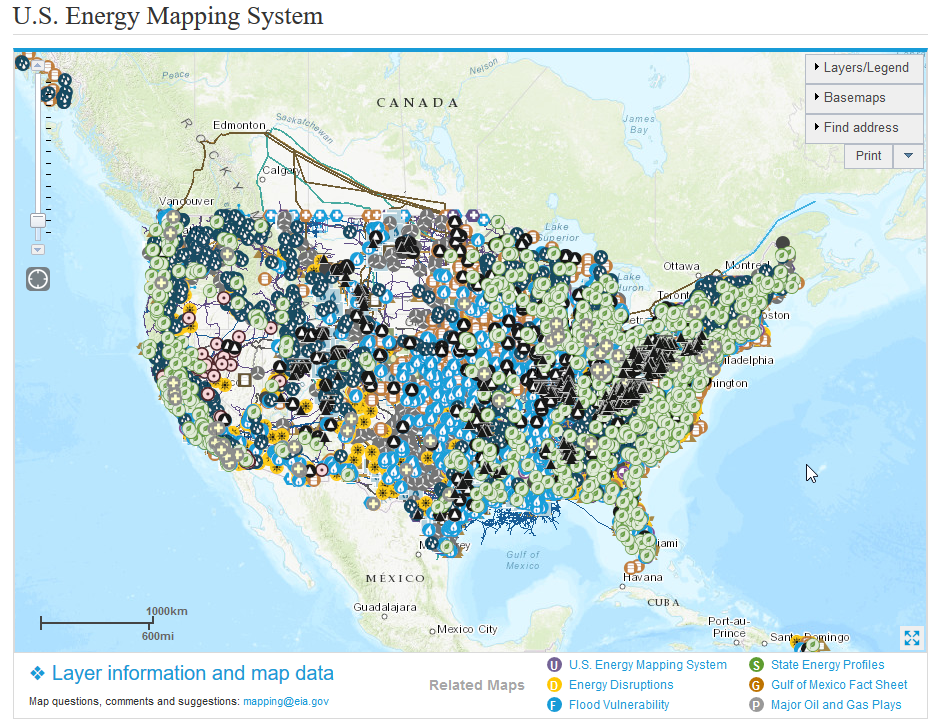
\includegraphics[width=0.8\linewidth]{images/eia_Example}
	\caption{EIA Mapping System Example}
	\label{fig:eiaexample}
\end{figure}


\subsubsection{Shortcomings:}
\begin{my_itemize}
	\item Poor interactivity and responsiveness
	\item Inability to display graphical data versus time
	\item Minimal and confusing data filtering options
	\item Low data-to-ink ratio
\end{my_itemize}


\subsection{How this is a new approach:}
We propose a set of interactive visualizations which will allow users to explore data from multiple sources on common media. \\

The success of our approach will require clear visuals which allow users to develop their own conclusions on climate impact, instead of being presented with a tailored narrative.  
\subsection{Who should care:} 
Climate change is a concern of individuals and organizations worldwide. More effective visualizations can reduce the awareness gap between scientific experts and the public.

\subsection{Measuring Success and Expected Impact:}
Success is measured by the effectiveness of our visualizations at conveying similar data as others while adding interactivity and blending of data sources. Impact is measured through user engagement and interaction.
\subsection{Risks}
\begin{my_itemize}
	\item Resource needs to process, clean, and present three large datasets
	\item Responsive performance for multiple visualizations on one page
	\item Geographic data granularity is insufficient to provide insights
\end{my_itemize}
\subsection{Payoffs}
\begin{my_itemize}
	\item Visualization provides real-world data for independent conclusions
	\item Climate insights from coal reduction and renewable expansion
	\item Sparks conversation and challenge around tailored climate data
\end{my_itemize}
\subsection{Costs}
\begin{my_itemize}
	\item Team time investment for data processing and visualizations
	\item Computational resources for large data set use
	\item Minimal monetary costs may be required for hosted solution
\end{my_itemize}

\newpage
\subsection{Measuring Progress:}
Progress will be measured against \textbf{Table \ref{table:actions}}. Weekly meetings are used to hold everyone accountable.  Individual effort will be monitored and appropriate actions taken.

\begin{table}[H] 
	\caption{Team 52 Actions}\label{table:actions}
\begin{tabular}{| p{1.75in} | c | >{\centering\arraybackslash}m{0.7in} |}

	\hline 
	\rowcolor{Gray}
	\textbf{Task} & \textbf{Due} & \textbf{Owner} \\ 
	\hline 
	Submit Progress Report & 3/29 & All \\
	\hline
	Begin Final Poster & 3/29 & All \\
	\hline
	Complete Final Poster & 4/12 & All \\
	\hline
	\rowcolor{Gray}
	\multicolumn{3}{|l|}{\textbf{The Data}} \\
	Download and clean CO$_2$ Dataset & 3/14 & D. Carvallo  \\ 
	\hline
	Download and clean Berekley weather dataset & 3/14 & W. Smith \\
	\hline
	Using EIA API pull power plant information & 3/14 & C. Comfort \& J. Bonifield \\
	\hline
	Combine datasets into a single database & 3/19 & All \\
	\hline
	\rowcolor{Gray}
	\multicolumn{3}{|l|}{\textbf{Visualizations}} \\
	Determine Visualization Platform (D3/Python/Tableau, etc) & 3/14 & All \\	
	\hline
	Base (non-dynamic) visualization working (either energy or climate only) & 3/26 & All \\
	\hline 
	Time Dependent visualization working & 4/2 & All \\
	\hline
	Full Visualization Working & 4/9 & All \\
	\hline
	\rowcolor{Gray}
	\multicolumn{3}{|l|}{\textbf{Completed Tasks}} \\
	Locate 2 possible datasets & Complete & All\\
	Locate 3 survey sources each & Complete & All \\
	Attend Tue and Thu Team Meetings & Complete & All\\
	\hline 
\end{tabular} 
\end{table}
\subsection{Checking Progress:}
The final exam will be a user test of the finalized visualization. The midterm check will be a cleaned, organized, and combined dataset organized geographically and a basic functioning visualization. 

\section{Literature Survey}
\subsection{CO$_2$ Emission Projections from Electrical Generation\\ \cite[Page Count:~11]{Comfort_1_Bruninx} and \cite[Page Count:~17]{Comfort_2_HammonsT2006IoEP}}
\textbf{Main Ideas:} Consisted of two papers which utilized climate modeling to predict CO$_2$ emissions based on energy production changes in Germany and Russia, Greece and Italy respectively.
\begin{figure}[H]
	\centering
	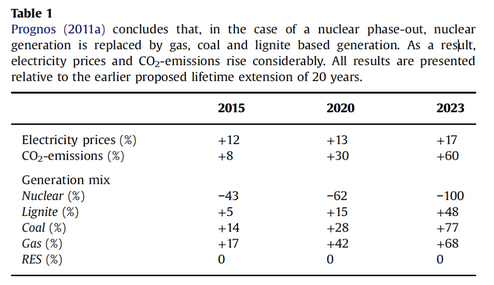
\includegraphics[width=0.9\linewidth]{images/co2ProjectTable}
	\caption{CO$_2$ Emission Impact Table \protect\cite{Comfort_1_Bruninx}}
	\label{fig:co2german}
\end{figure}

\textbf{Uses:} There is an overall correlation between CO$_2$ emissions and energy production.  The larger the percentage of low (or zero) CO$_2$ plants the lower overall CO$_2$ concentrations were predicted. \\

\textbf{Shortcoming:} CO$_2$ concentration results were projected to show a future state while our proposal focuses on measured data.\\

\subsection{Contemporary Climatic Analogs for 540 North American urban areas in the late 21st century \cite[Page Count:~7]{Comfort_4_FitzpatrickMatthew2019Ccaf}}
\textbf{Main Idea:} This survey developed analysis and visualization techniques that link current contemporary urban area climate-analogs to predict how future conditions in other urban areas may be similar.\\

\textbf{Uses:} It provides an interesting visualization approach through connecting similar climate areas in an effort to provide context to future climate change.  

\textbf{Shortcomings:} In some cases (\textbf{Table \ref{fig:connectedAnalog}}) the visualization becomes very busy connecting urban areas.\\
\begin{figure}[H]
	\centering
	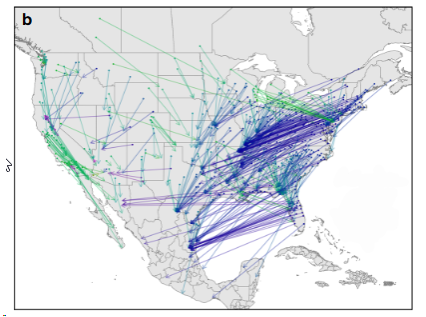
\includegraphics[width=0.9\linewidth]{images/connectedAnalog}
	\caption{Urban Area Connected Analog \protect\cite{Comfort_4_FitzpatrickMatthew2019Ccaf}}
	\label{fig:connectedAnalog}
\end{figure}

\subsection{Prospective Analysis of Life-Cycle Indicators through Endogenous Integration into a National Power Generation Model \cite[Page Count:~17]{Endogenous_resources5040039}}
\textbf{Main Idea:}Due to the lack of integration between Energy systems modeling and life cycle modeling, the authors of the report combined the two into one model to be utilized for forecasting. Their final proved to be useful in energy forecasting decision making.  \\
\begin{figure}[H]
	\centering
	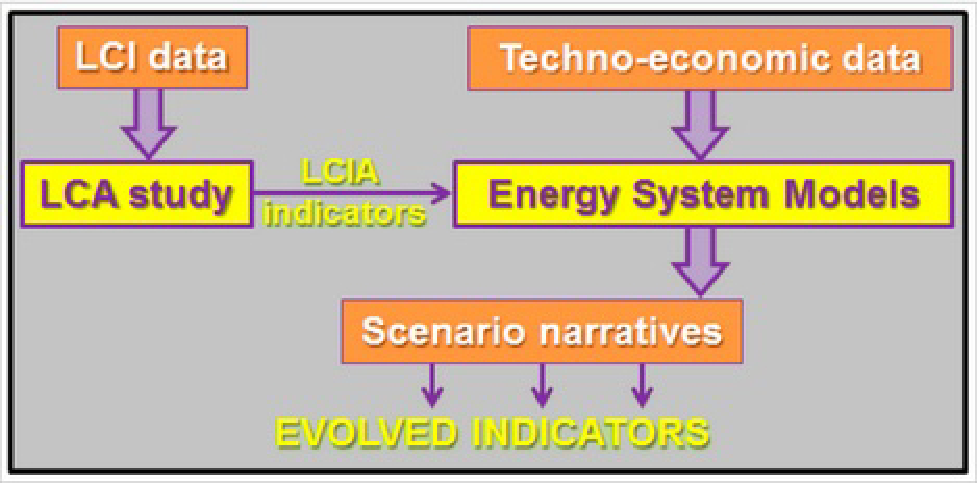
\includegraphics[width=0.7\linewidth]{images/endogenousFig}
	\caption{Merging LCA and ESM Approach \protect\cite{Endogenous_resources5040039}}
	\label{fig:endogenous}
\end{figure}
\textbf{Uses:} Proves the need to integrate energy data with climate data. Further, it provides an example of an existing model that combined both for forecasting reasons.  \\

\textbf{Shortcomings:} Their model is specific to the Spanish energy market end focuses solely on one major climate indicator and simplifies energy production into three main sources (nuclear, renewable and fossil).  

\subsection{The global climate change and its effect on power generation in Bangladesh  \cite[Page Count:~10]{Bangladesh_KHAN20131460}}
\textbf{Main Idea:} Energy sources in developing countries are more susceptible to different climate effects. Unless stopped, current trends estimate the effects of climate change to exponentially increase with time. \\

\textbf{Uses:} Provides examples of major climate factors that affect power generation and describes a need to reduce the effects of climate change.  \\

\textbf{Shortcomings:} Data is specific to Bangladesh and smaller countries. Model presented extrapolates climate change effects which may be unrealistic.\\
\begin{figure}[H]
	\centering
	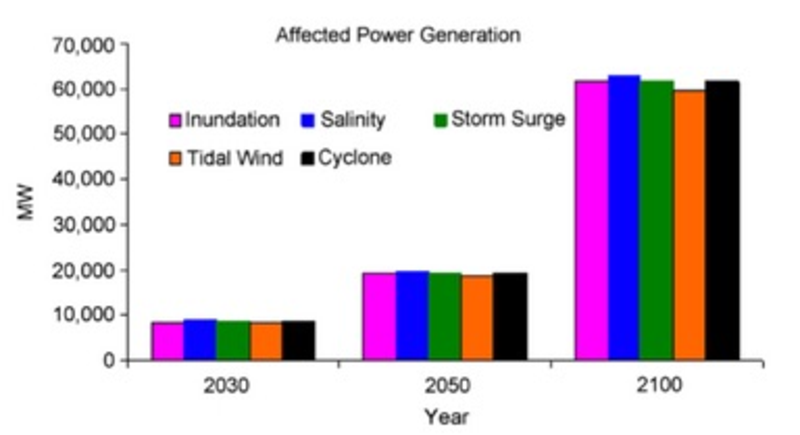
\includegraphics[width=0.7\linewidth]{images/bangladeshBar}
	\caption{Affected power generation by climate change till 2100 \protect\cite{Western_Europe_GolombekRolf2012Ccio}}
	\label{fig:westerEuropeBar}
\end{figure}

\subsection{Climate Change: Impacts on Electricity Markets in Western Europe \cite[Page Count:~14]{Western_Europe_GolombekRolf2012Ccio}}
\textbf{Main Idea:} Quantifies the effects of temperature and precipitation for electricity markets in Western Europe. \\

\textbf{Uses:} Paper provides quantifiable values which can be compared to values in our visualization to determine world-wide differences.\\

\textbf{Shortcomings:}  Large model variability in countries depending on generation production split.\\


\subsection{Reflections—What Would It Take to Reduce U.S. Greenhouse Gas Emissions 80 Percent by 2050? \cite[Page Count:~16]{reduce_greenhouse_rex014}}
\textbf{Main Idea:} Details the path to reducing CO2 emissions by 80\% by 2050. The greatest potential improvement being by replacement coal and gas with wind and solar. \\

\textbf{Uses:}  The analysis and projections of the author can inform our visualizations of trends in recent capacity across differing electricity production sectors. \\

\textbf{Shortcomings:}  Ignores the emission-reducing effects of other generation methods such as nuclear. \\

\subsection{Visualization of Climate and Climate Change Data: An Overview \cite[Page Count:~6]{Overview_article}}
\textbf{Main Idea:}  The effective visualization of Climate Change is essential. Surveys climate scientists and researchers on most used visualization strategies and software, and seeks to bridge the gap between cutting-edge climate and visualization research. \\

\textbf{Uses:}  The results and analysis of this usage research can help the team craft a more effective visualization.\\

\textbf{Shortcomings:}  Places insufficient emphasis on interactivity.\\

\subsection{Visualizing Climate change Risk and Adaptation Options for California \cite[Page Count:~24]{California_Report}}
\textbf{Main Idea:}  California is particularly sensitive to climate disruption. Visualization tools are critical to communicating the risks to local communities. \\

\textbf{Uses:} The results and analysis of this usage research can help the team craft a more effective visualization.  \\

\textbf{Shortcomings:} California specific focus limits general applicability. \\

\subsection{Visualising the potential impacts of climate change on rural landscapes \cite[Page Count:~23]{Rural_Landscape_DockertyTrudie2005Vtpi}}
\textbf{Main Idea:}  Broad visualizations of climate change are often not as effective at communicating a message as specifically tailored local approaches. By using a GIS database combined with photorealistic software and scenarios powered by decision rules specific the impact on specific communities \\

\textbf{Uses:} The results and analysis of this usage research can help the team craft a more effective visualization with respect to scenario modeling.  \\

\textbf{Shortcomings:}  Difficult to scale local approaches to all communities due to high variance in geographic/climate factors.         \\

\subsection{CO$_2$ Emission Trends for the US and Electric Power Sector \cite[Page Count:~14]{Emission_trend_KLEIN201633}}
\textbf{Main Idea:} The US has made remarkable progress recently in reducing CO2 emissions. From 2005-2012, more CO2 reduction occurred in the US than in all other countries combined. Electric power generation was the greatest contributor to this decline. \\

\textbf{Uses:} Contains very relevant data for our research detailing the effects of power generation mix on CO2 emissions.  \\

\textbf{Shortcomings:} Many visualizations are used which suffer from the same problems discussed elsewhere. We aim to bring this same data to life by adding interactivity.  \\

\subsection{Climate Change 2013: The Physical Science Basis, Chapter 2 \cite[Page Count:~90]{Climate_change_2013_stocker2014climate}}
\textbf{Main Idea:} Provides a complete survey of recent results in climate science across a broad range of sources with a wealth of visual content. A central finding since previous reports is that there is widespread agreement in temperature increase estimates among the various temperature datasets.  \\

\textbf{Uses:} Inform our understanding of state-of-the-art techniques in climatology on a global scale, specifically with respect to atmosphere and surface.  \\

\textbf{Shortcomings:} Visualizations lack interactivity and are often jargon-heavy, failing to highlight recent findings adequately for observers with little domain knowledge.   \\

%**********
\section{Team Member Effort:}
All team members have contributed equally to the project.
% The next two lines define the bibliography style to be used, and the bibliography file.

\section{Word Count - See Appendix}

\bibliographystyle{ACM-Reference-Format}
\bibliography{proposal_references}

% 
% If your work has an appendix, this is the place to put it.
\onecolumn
\newpage
\section*{Appendix - Word Count}

\begin{figure}[H]
	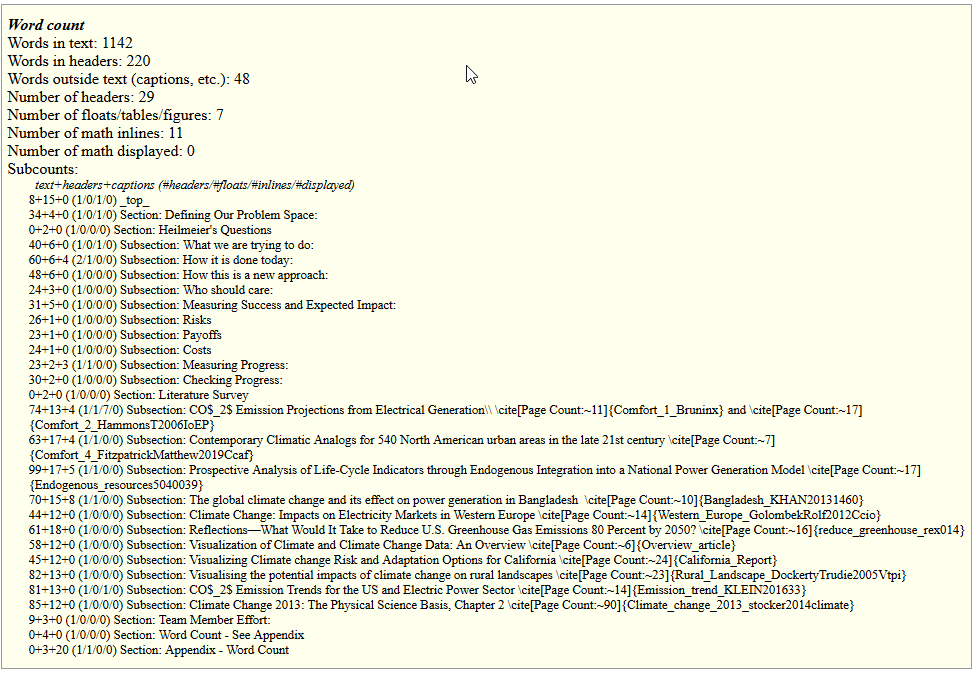
\includegraphics[width=0.9\linewidth]{images/wordCount}
	\caption{The word count for this document, including this section is: 1142 using \href{https://app.uio.no/ifi/texcount/online.php}{\color{blue}TeXCount Web Service}.}\label{fig:wordCount}
\end{figure}

\end{document}
